\subsection{Reactions}

\subsubsection{Solution}
Source: \href{https://www.youtube.com/watch?v=AN4KifV12DA&list=PL8dPuuaLjXtPHzzYuWy6fYEaX9mQQ8oGr&index=8}{Water \& Solutions - for Dirty Laundry: Crash Course Chemistry \#7}

\begin{description}
    \item[] solute in solvent = solution 
    \item[] water is polar \arrow great solvent \arrow aqueous solution
    \item[] similar dissolve
    \begin{description}
        \item[polar] water \arrow hydrophilic, lipophobic
        \item[non-polar] fat \arrow lipophilic, hydrophobic
    \end{description}
    \item[] ions in solution are electrolytes \arrow salts make water conductive \arrow dielectric property
    \item[] hydration energy $>$ lattice energy \arrow enthalpy is negative \arrow heat is released
    \item[] hydration energy $<$ lattice energy \arrow enthalpy is positive \arrow heat is absorbed
\end{description}

\subsubsection{Acid-Base}
Source: \href{https://www.youtube.com/watch?v=ANi709MYnWg&list=PL8dPuuaLjXtPHzzYuWy6fYEaX9mQQ8oGr&index=9}{Acid-Base Reactions in Solution: Crash Course Chemistry \#8}

\begin{description}
    \item[acid] anything that donates a Proton
    \item[base] anything that accepts a Proton 
    \item[$\text{H}^+$] Protons in solution \arrow Hydrogen atom without electron \arrow Hydronium \arrow Proton
    \item[Conjugate acid] $\text{H}_3\text{O}^+ \qquad \text{N}\text{H}_4^+$ 
    \item[Conjugate base] $\text{C}\text{L}^- \qquad \text{O}\text{H}^-$ 
\end{description}

\subsubsection{Precipitation}
Source: \href{https://www.youtube.com/watch?v=IIu16dy3ThI&list=PL8dPuuaLjXtPHzzYuWy6fYEaX9mQQ8oGr&index=10}{Precipitation Reactions: Crash Course Chemistry \#9}
\\
Stuff falling out of other stuff as solid precipitate!\\
$\text{AgNO}_{3(aq)}+\text{NaCl}_{(aq)} \to \text{NaNo}_{3(aq)} + \text{AgCl}_{(s)}$
\subsubsection{Redox}
Source: \href{https://www.youtube.com/watch?v=lQ6FBA1HM3s&list=PL8dPuuaLjXtPHzzYuWy6fYEaX9mQQ8oGr&index=11}{Redox Reactions: Crash Course Chemistry \#10}
\\
OIL RIG = Oxidation Is Loss of electrons, Redux Is Gain of electrons\\

\begin{description}
    \item[1] Elements by themselves have an oxidation state of 0.
    \item[2] Monatomic ion has its charge already (Cl$^-$).
    \item[3] Oxygen has an oxidation state of -II (Except Peroxides, H$_2$O$_2$).
    \item[4] Hydrogen has an oxidation state of -I (Except Hydriden, NaH).
    \item[5] Fluorine is -I
    \item[6] Metal always have a positive oxidation state. 
\end{description}

\subsubsection{Electrical current in salty solutions}

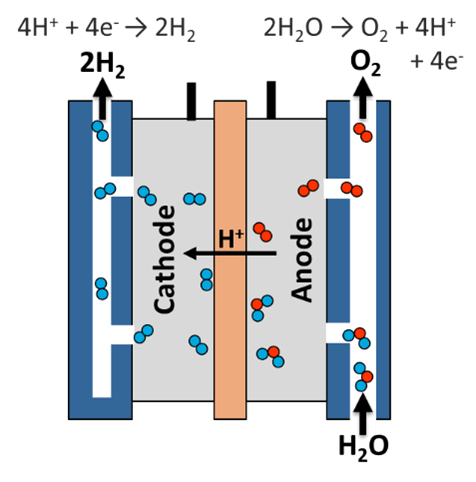
\includegraphics{./includes/chemistry/imgs/electrolyzer.png}
\\
Here the electrons flow from the Cathode- to the Anode+ (Through the wire).\\
The protons H+ flow from the Anode to the Cathode (through the electrolyte).